%% This is file `elsarticle-template-1-num.tex',
%%
%% Copyright 2009 Elsevier Ltd
%%
%% This file is part of the 'Elsarticle Bundle'.
%% ---------------------------------------------
%%
%% It may be distributed under the conditions of the LaTeX Project Public
%% License, either version 1.2 of this license or (at your option) any
%% later version.  The latest version of this license is in
%%    http://www.latex-project.org/lppl.txt
%% and version 1.2 or later is part of all distributions of LaTeX
%% version 1999/12/01 or later.
%%
%% Template article for Elsevier's document class `elsarticle'
%% with numbered style bibliographic references
%%
%% $Id: elsarticle-template-1-num.tex 149 2009-10-08 05:01:15Z rishi $
%% $URL: http://lenova.river-valley.com/svn/elsbst/trunk/elsarticle-template-1-num.tex $
%%
\documentclass[preprint,12pt]{elsarticle}

%% Use the option review to obtain double line spacing
%% \documentclass[preprint,review,12pt]{elsarticle}

%% Use the options 1p,twocolumn; 3p; 3p,twocolumn; 5p; or 5p,twocolumn
%% for a journal layout:
%% \documentclass[final,1p,times]{elsarticle}
%% \documentclass[final,1p,times,twocolumn]{elsarticle}
%% \documentclass[final,3p,times]{elsarticle}
%% \documentclass[final,3p,times,twocolumn]{elsarticle}
%% \documentclass[final,5p,times]{elsarticle}
%% \documentclass[final,5p,times,twocolumn]{elsarticle}

%% The graphicx package provides the includegraphics command.
\usepackage{graphicx}
%% The amssymb package provides various useful mathematical symbols
\usepackage{amssymb}
%% The amsthm package provides extended theorem environments
%% \usepackage{amsthm}

%% The lineno packages adds line numbers. Start line numbering with
%% \begin{linenumbers}, end it with \end{linenumbers}. Or switch it on
%% for the whole article with \linenumbers after \end{frontmatter}.
\usepackage{lineno}

%% natbib.sty is loaded by default. However, natbib options can be
%% provided with \biboptions{...} command. Following options are
%% valid:

%%   round  -  round parentheses are used (default)
%%   square -  square brackets are used   [option]
%%   curly  -  curly braces are used      {option}
%%   angle  -  angle brackets are used    <option>
%%   semicolon  -  multiple citations separated by semi-colon
%%   colon  - same as semicolon, an earlier confusion
%%   comma  -  separated by comma
%%   numbers-  selects numerical citations
%%   super  -  numerical citations as superscripts
%%   sort   -  sorts multiple citations according to order in ref. list
%%   sort&compress   -  like sort, but also compresses numerical citations
%%   compress - compresses without sorting
%%
%% \biboptions{comma,round}

% \biboptions{}

\journal{Journal Name}

\begin{document}

\begin{frontmatter}

%% Title, authors and addresses

\title{Unnecessarily Complicated Research Title}

%% use the tnoteref command within \title for footnotes;
%% use the tnotetext command for the associated footnote;
%% use the fnref command within \author or \address for footnotes;
%% use the fntext command for the associated footnote;
%% use the corref command within \author for corresponding author footnotes;
%% use the cortext command for the associated footnote;
%% use the ead command for the email address,
%% and the form \ead[url] for the home page:
%%
%% \title{Title\tnoteref{label1}}
%% \tnotetext[label1]{}
%% \author{Name\corref{cor1}\fnref{label2}}
%% \ead{email address}
%% \ead[url]{home page}
%% \fntext[label2]{}
%% \cortext[cor1]{}
%% \address{Address\fnref{label3}}
%% \fntext[label3]{}


%% use optional labels to link authors explicitly to addresses:
%% \author[label1,label2]{<author name>}
%% \address[label1]{<address>}
%% \address[label2]{<address>}

\author{John Smith}

\address{California, United States}

\begin{abstract}
%% Text of abstract

\end{abstract}

\begin{keyword}
Science \sep Publication \sep Complicated
%% keywords here, in the form: keyword \sep keyword

%% MSC codes here, in the form: \MSC code \sep code
%% or \MSC[2008] code \sep code (2000 is the default)

\end{keyword}

\end{frontmatter}

%%
%% Start line numbering here if you want
%%
\linenumbers

%% main text
\section{Introduction}
\label{S:1}

\begin{itemize}
\item Risk and uncertainty
\item One rule for all?
\item Impact of life histories
\item Comparision of constant catch v changing catch based on trends in an empirical index. 
\item catch only - need good catch data if you havent got this how can you set catch limits
\end{itemize}

Sustainability and risks to non target exploited marine fish stock populations requires both estimates of current stock status, the effects of fishing pressure (catchability and fishing effort) and the effects of management measures on target populations, however these data are often lacking.  Subsequently there is increasing concern and a growing need for the development of innovative approaches so that management of all marine stocks not just those of high commercial value can be included into the Common Fisheries Policy (CFP \cite{european2013regulation}) framework. Under the CFP management objectives are to recover stocks and to maintain stocks within safe biological limits to levels that can produce Maximum Sustainable Yield (MSY), including by-catch species by 2015 (Implementation Plan adopted at the World Summit on Sustainable Development, Johannesburg in 2002) and no later than 2020. These conservation objectives are currently being achieved by introducing biological target (can fluctuate around targets) and limit (i.e must not be exceeded) reference points e.g. population size (stock biomass) and/or yields (catches) and/or long–term yields and fishing mortality against which the preservation of stocks within such limits are assessed. These targets or limit reference points are often referred to as harvesting strategies which include an operational component called a harvest control rule (HCR) that are based on indicators (e.g. monitoring data or models) of stock status and to prevent overfishing. 

The International Council for the Exploration of the Sea (ICES) categorises stocks in to classes \emph{data-rich}, (categories 1 and 2) i.e those that have a quantitive assessment based on conventional mehods that require large amounts of data that include a long historical time series of catches and sound biological information \cite{bentley2015data}; or \emph{data-limted} \cite{costello2012status}(categories 3 and 4) (often called data poor) those without assessment, forecasts and have limited funding for research. For data-rich stocks ICES uses two types of reference points for providing fisheries advice; 
\begin{enumerate}
  \item Precautionary Approach (PA) reference points (those relating to stock status and exploitation relative to precautionary objectives) and 
  \item MSY reference points (those relating to achieving MSY) 
\end{enumerate}
In contrast for data limited stocks MSY \emph{proxy} reference points are used to estimate stock status and exploitation.  Often many of the methods used to estimate MSY proxy reference points require length based inputs as they are cheap, easy to collect \cite{quinn1999quantitative} and are related to life history paramters such as fish size, mortality and fecundity as well as fishery selectivity. For example many methods are being developed to estimate MSY, but currently only 4 are approved by ICES, these include, Surplus Production model in Continuous Time (catch based) (SPiCT; \cite{pedersen2017stochastic}, Mean Length Z (MLZ; \cite{gedamke2006estimating}), Length Based Spawner Per Recruit (LBSPR; \cite{hordyk2014some}) and Length Based Indicators (LBI; e.g. \cite{probst2013indicator}). The aforementoned data limited procedures have differing data requirements, intended uses and obviously have their own strengths and weaknesses. 

To test the performance of candidate management procedures often requires evaluation of alternative hypothesis about the dynamics of the system e.g. population dynamics (life history dynamics such as growth parameters which are an indication of fishery exploitation levels and management) and the behaviour of the fishery (e.g range contraction and density dependence) etc.. Due to the nature of conflicting objectives, stakeholder interests and the uncertainty in the dynamics of the resource and/ or the plausibility of alternative hypotheses can lead to poor decision making and can be problematic when defining management policy.

An intense area of work being researched over the last 2 decades is Management Strategy Evaluation (MSE), which focuses on the broader aspects of fishing (the Ecosystem) whereby different management options are tested against a range of objectives (see \cite{kell2007flr}. The approach is not to come up with a definitive answer, but to lay-bare the trade offs associated with each management objective, along with identifying and incorporating uncertainties in the evaluation and communicating the results effectively to client groups and decision-makers. MSE is not intended to be complex but to provide a robust framework that account for conflicting poorly defined objectives and uncertainties that have been absent in conventional management \cite{kell2007flr}. 

To assess case specific harvest strategies (via simulation) within the MSE, we will implement a management procedure based on a empirical HCR that adjusts yield depending on stock status for a given set of tunable parameters for each of the harvest strategies and to test their robustness to uncertainty.  This approach could also help identify similar conditions across species where particular advice rules are likely to work well, and where they perform poorly for a given a set of parameters. 

Often empirical harvest control rules require extensive exhaustive parameter searches to tune or optimise 'hyper-parameters' (external parameters to a model) that aren’t directly learnt from estimators.  This requires a technique known as a grid search that extensively searches for all combinations of all parameters. In contrast, and some what less time consuming alternative and efficient parameter search strategies can be considered for a given range of parameter space and a known distribution.  As such a random sample can be obtained and used to perform the different experiments for parameter optimisation. This approach differs from the simplest constant catch HCR strategy whereby catches are kept constant and low to ensure no lasting damage is done in periods of low stock productivity or whereby the stock is highly variable year on year, therefore the empirical approach can help optimise catch by setting a precautionary Total Allowable Catch (TAC). 

Here we describe methods to assess the performance of each empirical HCR via a set of utilities and show the benefits compared to a constant catch strategy across a spectrum of different species: safety ($B/B_{MSY} >1$), yield ($yield/MSY$), kobe proportion (proportion of years that stay in the green zone of kobe plot ($B/B_{MSY} >1$), and Yield Annual Variation (yield changes by 10\% year on year). 


\section{Material and Methods}
\subsection{Materials}


Life history parameters for growth, natural mortality and maturity were used to develop an age-based Operating Model. To do this the parameters were first used to parameterise functional forms for mass ($W$), proportion mature ($Q$), natural mortality ($M$) and fishing mortality ($F$) at age. These were then used to calculate the  spawner ($S/R$) and yield-per-recruit ($Y/R$) which were then combined with a stock recruitment relationship \cite{sissenwine1987alternative} to calculate the equilibrium stock size as a function of fishing mortality ($F$). 

This analysis allows a variety of reference points such as those based on Maximum Sustainable Yield ($MSY$), i.e. $B_{MSY}$ the spawning stock biomass ($S$) and $F_{MSY}$ the fishing mortality that produces $MSY$ at equilibrium to be estimated. Other reference points are $F_{0.1}$ the fishing mortality on the yield per recruit curve where the slope is 10\% of that at the origin, a conservative proxy for $F_{MSY}$; and
$F_{Crash}$ which is the fishing mortality that will drive the stock to extinction since it is equivalent to a $R/S$ greater than the slope at the origin of the stock recruitment relationship, i.e. recruitment can not replace removals for a fishing mortality equal to $F_{Crash}$.  

The equilibrium relationships can then be turned into a forward dynamic model and projected forward.

A variety of functional forms can be assumed for all of the various process, i.e. growth, mortality, maturity, the selection pattern of the fisheries and the stock recruitment relationship. Commonly processes such as growth an maturity-at-age are well known while those for natural mortality and the stock recruitment relationship are poorly known \cite{michielsens2004bayesian}. In the later case assumptions have to be made and to evaluate the sensitivity of any analysis to those assumptions a variety of scenarios are considered. 

\subsection{Methods}

Individual Growth

Growth in length is modelled by the Von Bertalanffy growth equation @vonbert1957quantitative

\begin{equation} L = L_\infty(1 - exp(-k(t-t_0)) \end{equation}
         
where $k$ is the rate at which the rate of growth in length declines as length approaches the asymptotic length  $L_\infty$ and $t_{0}$ is the hypothetical time at which an individual is of zero length.

Length is converted to mass using the length-weight relationship 
    
\begin{equation} W = aL_t^b \end{equation}

\noindent where $a$ is the condition factor and $b$ is the allometric growth coefficient.


Maturity-at-age

Proportion mature-at-age is modelled by the logistic equation with 2 parameters: age at 50\% ($a_{50}$) and 95\% ($a_{95}$) mature.

\begin{equation}
f(x) = \left\{ \begin{array}{ll}
			0                                 &\mbox{ if $(a_{50}-x)/a_{95} >  5$} \\
			a_{\infty}                        &\mbox{ if $(a_{50}-x)/a_{95} < -5$} \\
			\frac{m_{\infty}}{1.0+19.0^{(a_{50}-x)/_{95})}} &\mbox{ otherwise}
		\end{array}
       \right.
\end{equation}


\subsubsection{Operating Model}

Age based.

\subsubsection{Management Procedure}

The management procedure was based on an empirical MP, where an increase in an index of abundance resulted in an increase in the TAC, while a decrease in the index results in an decrease in the TAC.

\subsubsection{Random Search}

%https://stats.stackexchange.com/questions/160479/practical-hyperparameter-optimization-random-vs-grid-search

When running an MSE commonly a set of MP scenarios are run to tune the MP, this requires running the MSE for each OM scenario for a range of fixed values in the HCR and then choosing the rule that best meets management objectives. If there are a lot of parameters to tune then a grid search may become unfeasible. An alternative is random search \cite{bergstra2012random} as randomly chosen trials are more efficient for parameter optimisation than trials based on a grid. 

%For example any distribution over a sample space with a finite maximum, the maximum of 60 random observations lies within the top 5\% of the true maximum, with 95\% probability.  Imagine the 5\% interval around the true maximum. Now imagine that we sample points from his space and see if any of it lands within that maximum. Each random draw has a 5\% chance of landing in that interval, if we draw n points independently, then the probability that all of them miss the desired interval is (1−0.05)n So the probability that at least one of them succeeds in hitting the interval is 1 minus that quantity. We want at least a .95 probability of success. To figure out the number of draws we need, just solve for n in the equation: 1−(1−0.05)^n>0.95 We get n⩾60
  
\section{Results}

Estimates of the simulated life history parameters obtained from Fishbase (http://www.fishbase.org) are presented in Fig.1. These show that for fast growing species which are small in size $l_{\infty}$ (asymtopic length parameter) species such as sprat, the growth parameter \textit{k} is high. The sprats age-at-50\%-maturity \textit{a50} are low, in contrast to a slower growing larger longer lived species $l_{\infty}$ such as rays or pollack.

Observations in Fig.2 shows that the assumed maturity in the OM is related to selectivity and that the faster growing species are more susceptible to fishing, although the slower growing larger (by mass and length) species (e.g. pollack has a higher natural mortality rate at lower ages) with the most significant rate increases associated with turbot. A levelling off in the mortality rate is evident for ray just prior to age 4.5. In contrast, there have been less steep declines in natural mortality estimates for brill, but most notably for sprat. 

Fig.3 displays the equilibrium relationships of the operating model. Comparisons of reference points estimates can be made across species.  The \textit{m/k} plot shows interesting trends with lower values for sprat where the growth rate \textit{k} is considerably higher than the natural mortality rate with little uncertainty around the estimate. In contrast to a slower growing species such as pollack where natural mortality is higher, as is the uncertainty around the estimate. The relationships when compared the proxy for fishing pressure \textit{f/m} show that the estimate is considerably higher in sprat than pollack, however the intrinsinc population growth rate \textit{r} shows that sprats reproductive capacity is higher and thus its surplus production. 


\textbf{[EXAMPLES TO BE UPDATED]}
\begin{itemize}
\item Figure \ref{fig:lh} shows the life history parameters
\item Figure \ref{fig:vector} shows the vectors
\item Figure \ref{fig:ts} shows the time series relative to reference points
\item Figure \ref{fig:pm} shows the performance statistics; points are
\begin{enumerate}
 \item ~
 \item ~
 \item ~
 \item ~\item Figure \ref{fig:util} shows the utility functions for the seven study stocks points area
\end{enumerate}
\begin{enumerate}
 \item ~
 \item ~
 \item ~
 \item ~
\end{enumerate}

\end{itemize}

\section{Discussion}

<<<<<<< HEAD
Fisheries management is often faced with multiple conflicting objectives e.g social, biological and economic, and it is widely recognised that their is a need to incorporate these objectives into management plans. Howvever such an experiment on large scale fish stocks is nearly impossible to perform.  Therefore performing computer simulations to develop robust management procedures is particularly valuable in data poor situtations where knowledge and data are limited, but also in data rich situtaions as simulation testing an assessment procedure using a model conditioned on the same assumptions is not necessarily a true test of robustness.  This paper has shown that the desired performance measure can be met via tweaking of the management procedure by adjusting a particular HCR a specific management objective an be achieved. Although the results of the various MSE analyses conditioned using a generic OM where fairly similar there was not a single advice rule to fit all species life-history types and fishery conditions. 

The application

=======
Fisheries management is often faced with multiple conflicting objectives e.g social, biological and economic, and it is widely recognised that their is a need to incorporate these objectives into management plans. Howvever such an experiment on large scale fish stocks is nearly impossible to perform.  Therefore performing computer simulations to develop robust management procedures is particularly valuable in data poor situtations where knowledge and data are limited, but also in data rich situtaions as simulation testing an assessment procedure using a model conditioned on the same assumptions is not necessarily a true test of robustness.  This paper has shown that the desired performance measure can be met via tweaking of the management procedure by adjusting a particular HCR a specific management objective an be achieved.
>>>>>>> 9f0ea9968a72580e1c183481446c56ba740ff800

\begin{itemize}
\item Bullet point one
\item Bullet point two
\end{itemize}

\section{Conclusions}
Further exploration of alternative advice rules, weightings of individual components within a generic advice rule, time-lags in data, and selection of amount of historical data to use, would be useful for identifying a suite of advice rules that perform well under the various fishery conditions of the ICES category 3 & 4 stocks.

\begin{itemize}
\item Bullet point one
\item Bullet point two
\end{itemize}

\section{References}

\bibliographystyle{model1-num-names}
\bibliography{/Users/alextidd/Documents/RandomGrid/tex/refs.bib} 

\section{Figures}

\begin{figure}[]\centering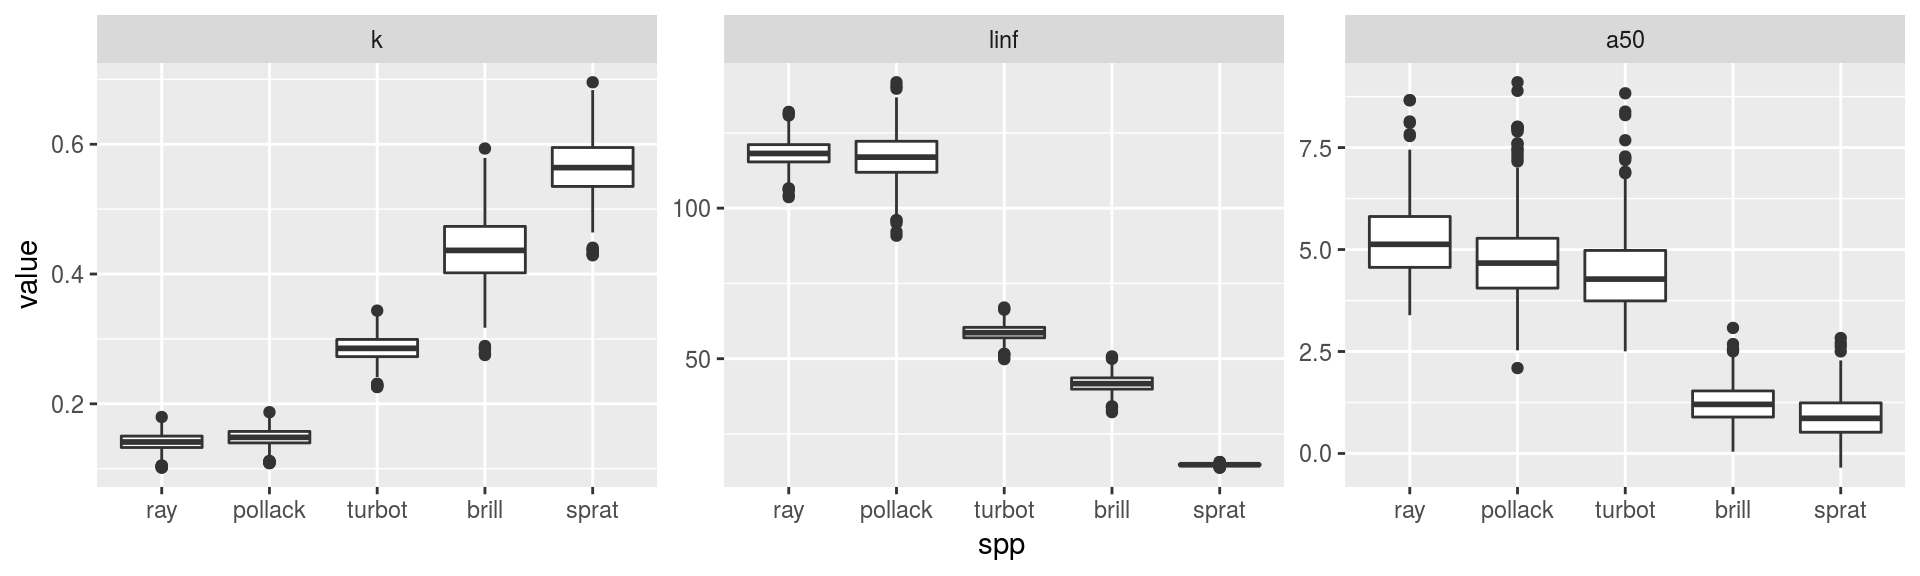
\includegraphics[width=5in]{rg-lhpar-1.png}\caption{}\label{fig:lh}\end{figure}
\begin{figure}[]\centering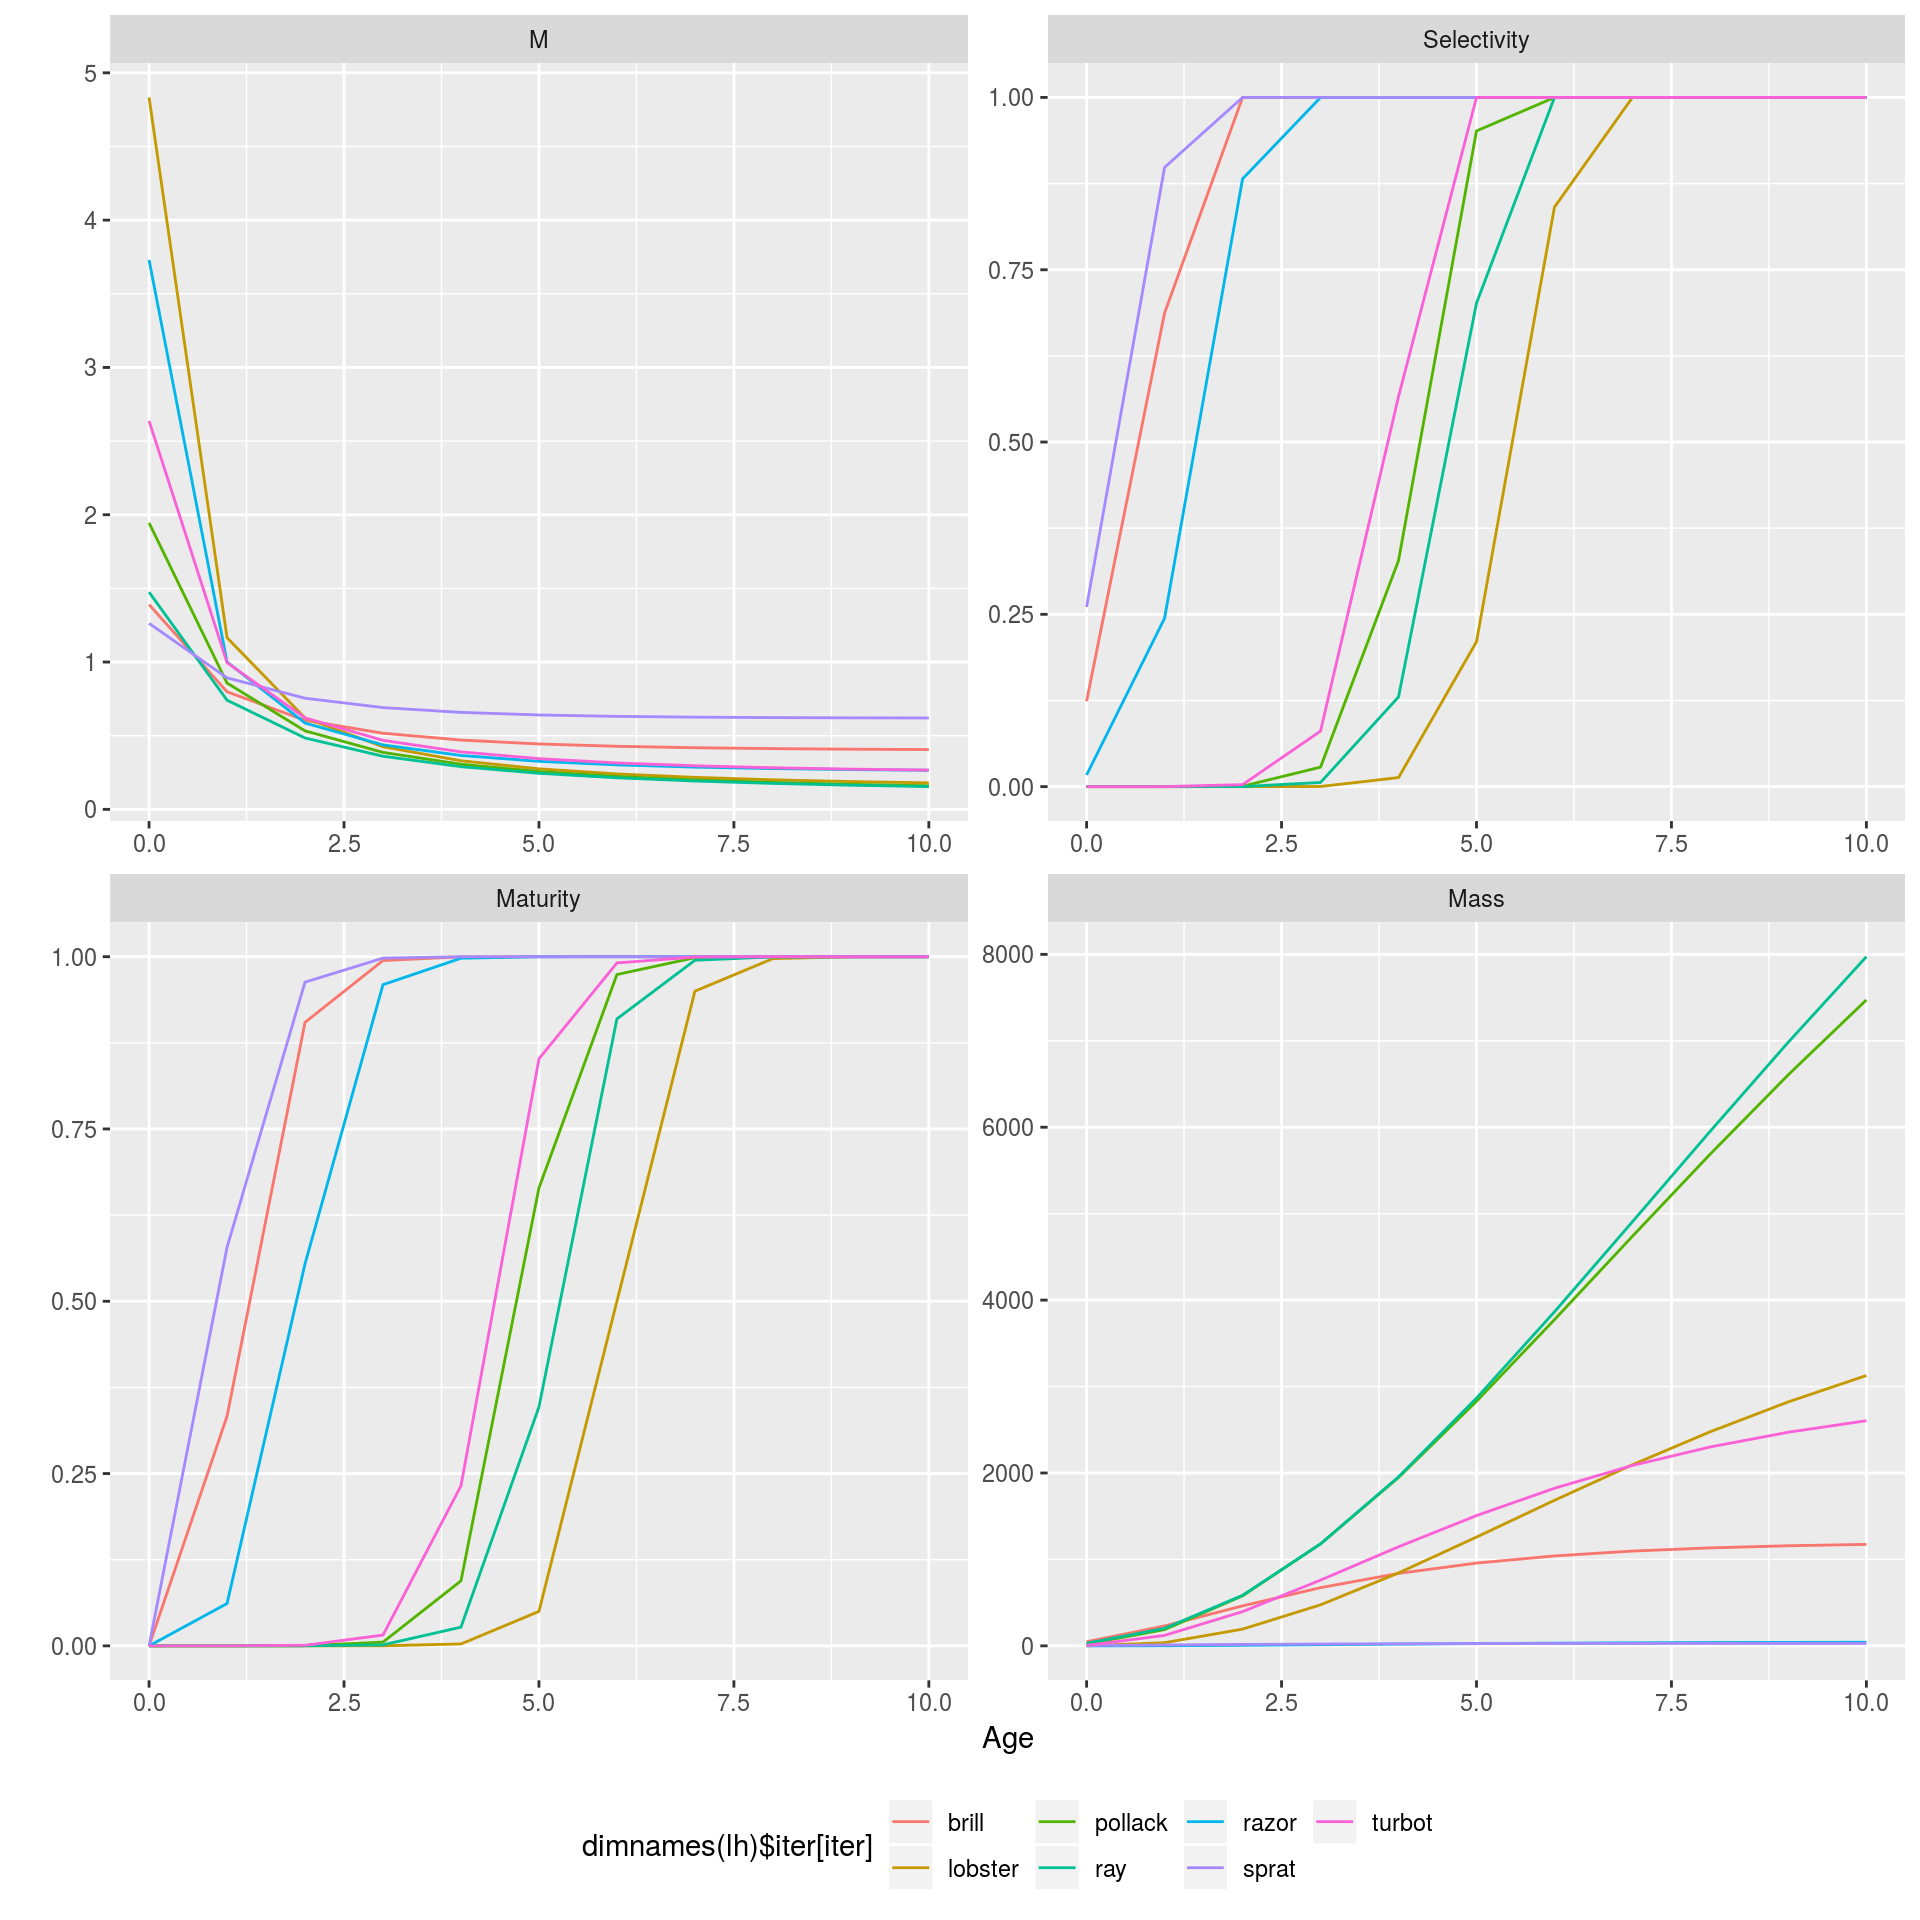
\includegraphics[width=5in]{rg-vectors-1.png}\caption{}\label{fig:vector}\end{figure}
\begin{figure}[]\centering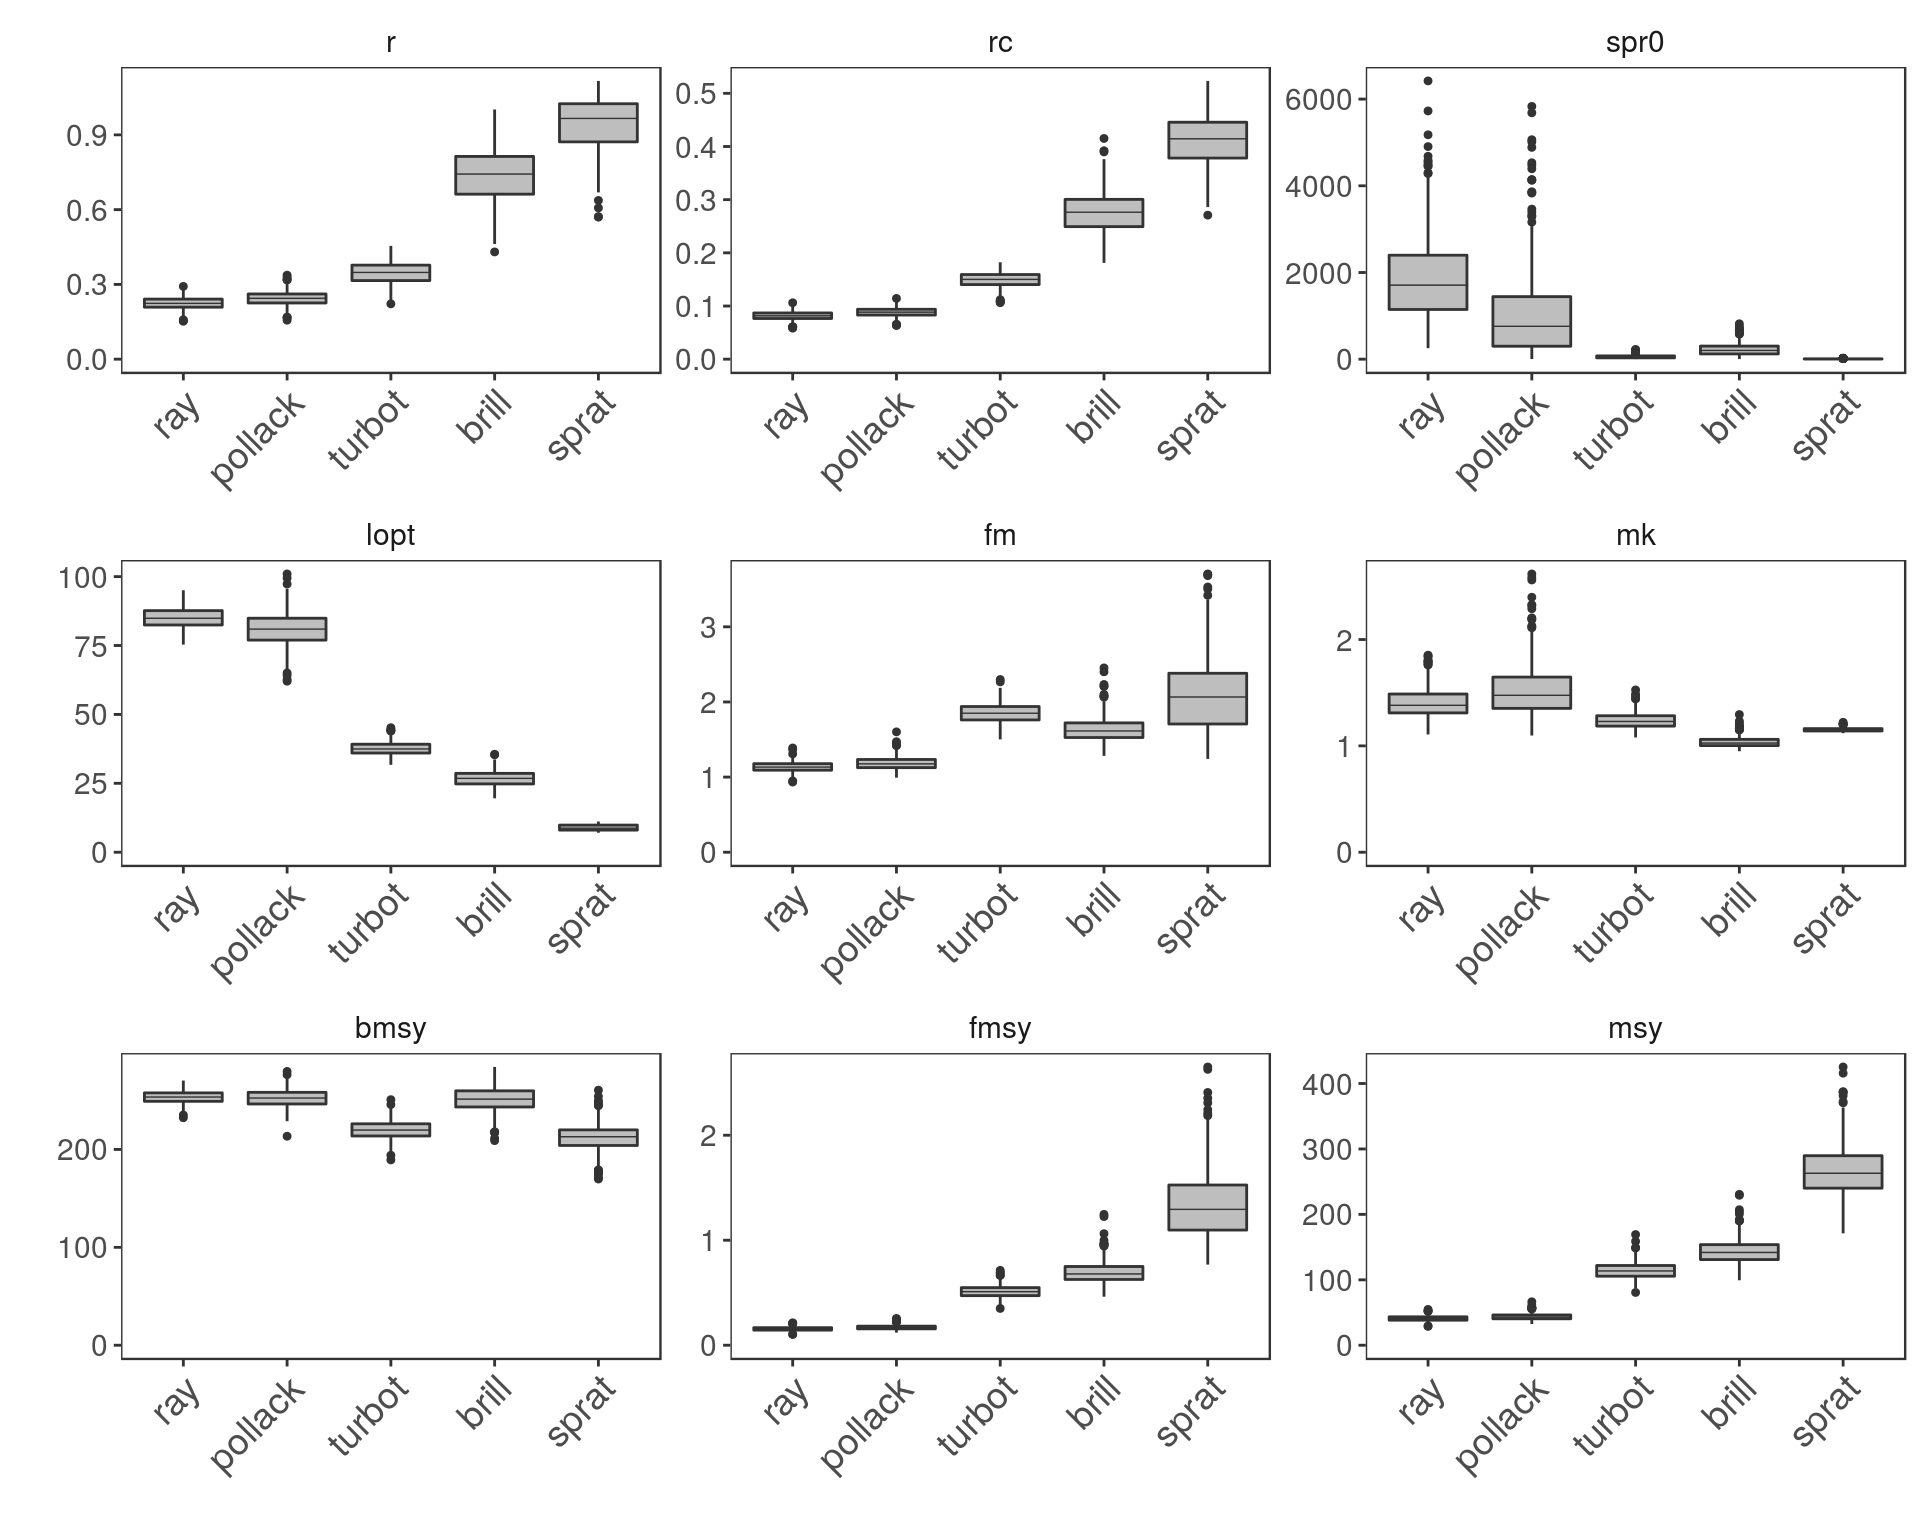
\includegraphics[width=5in]{rg-derived-1.png}\caption{}\label{fig:lh}\end{figure}
\begin{figure}[]\centering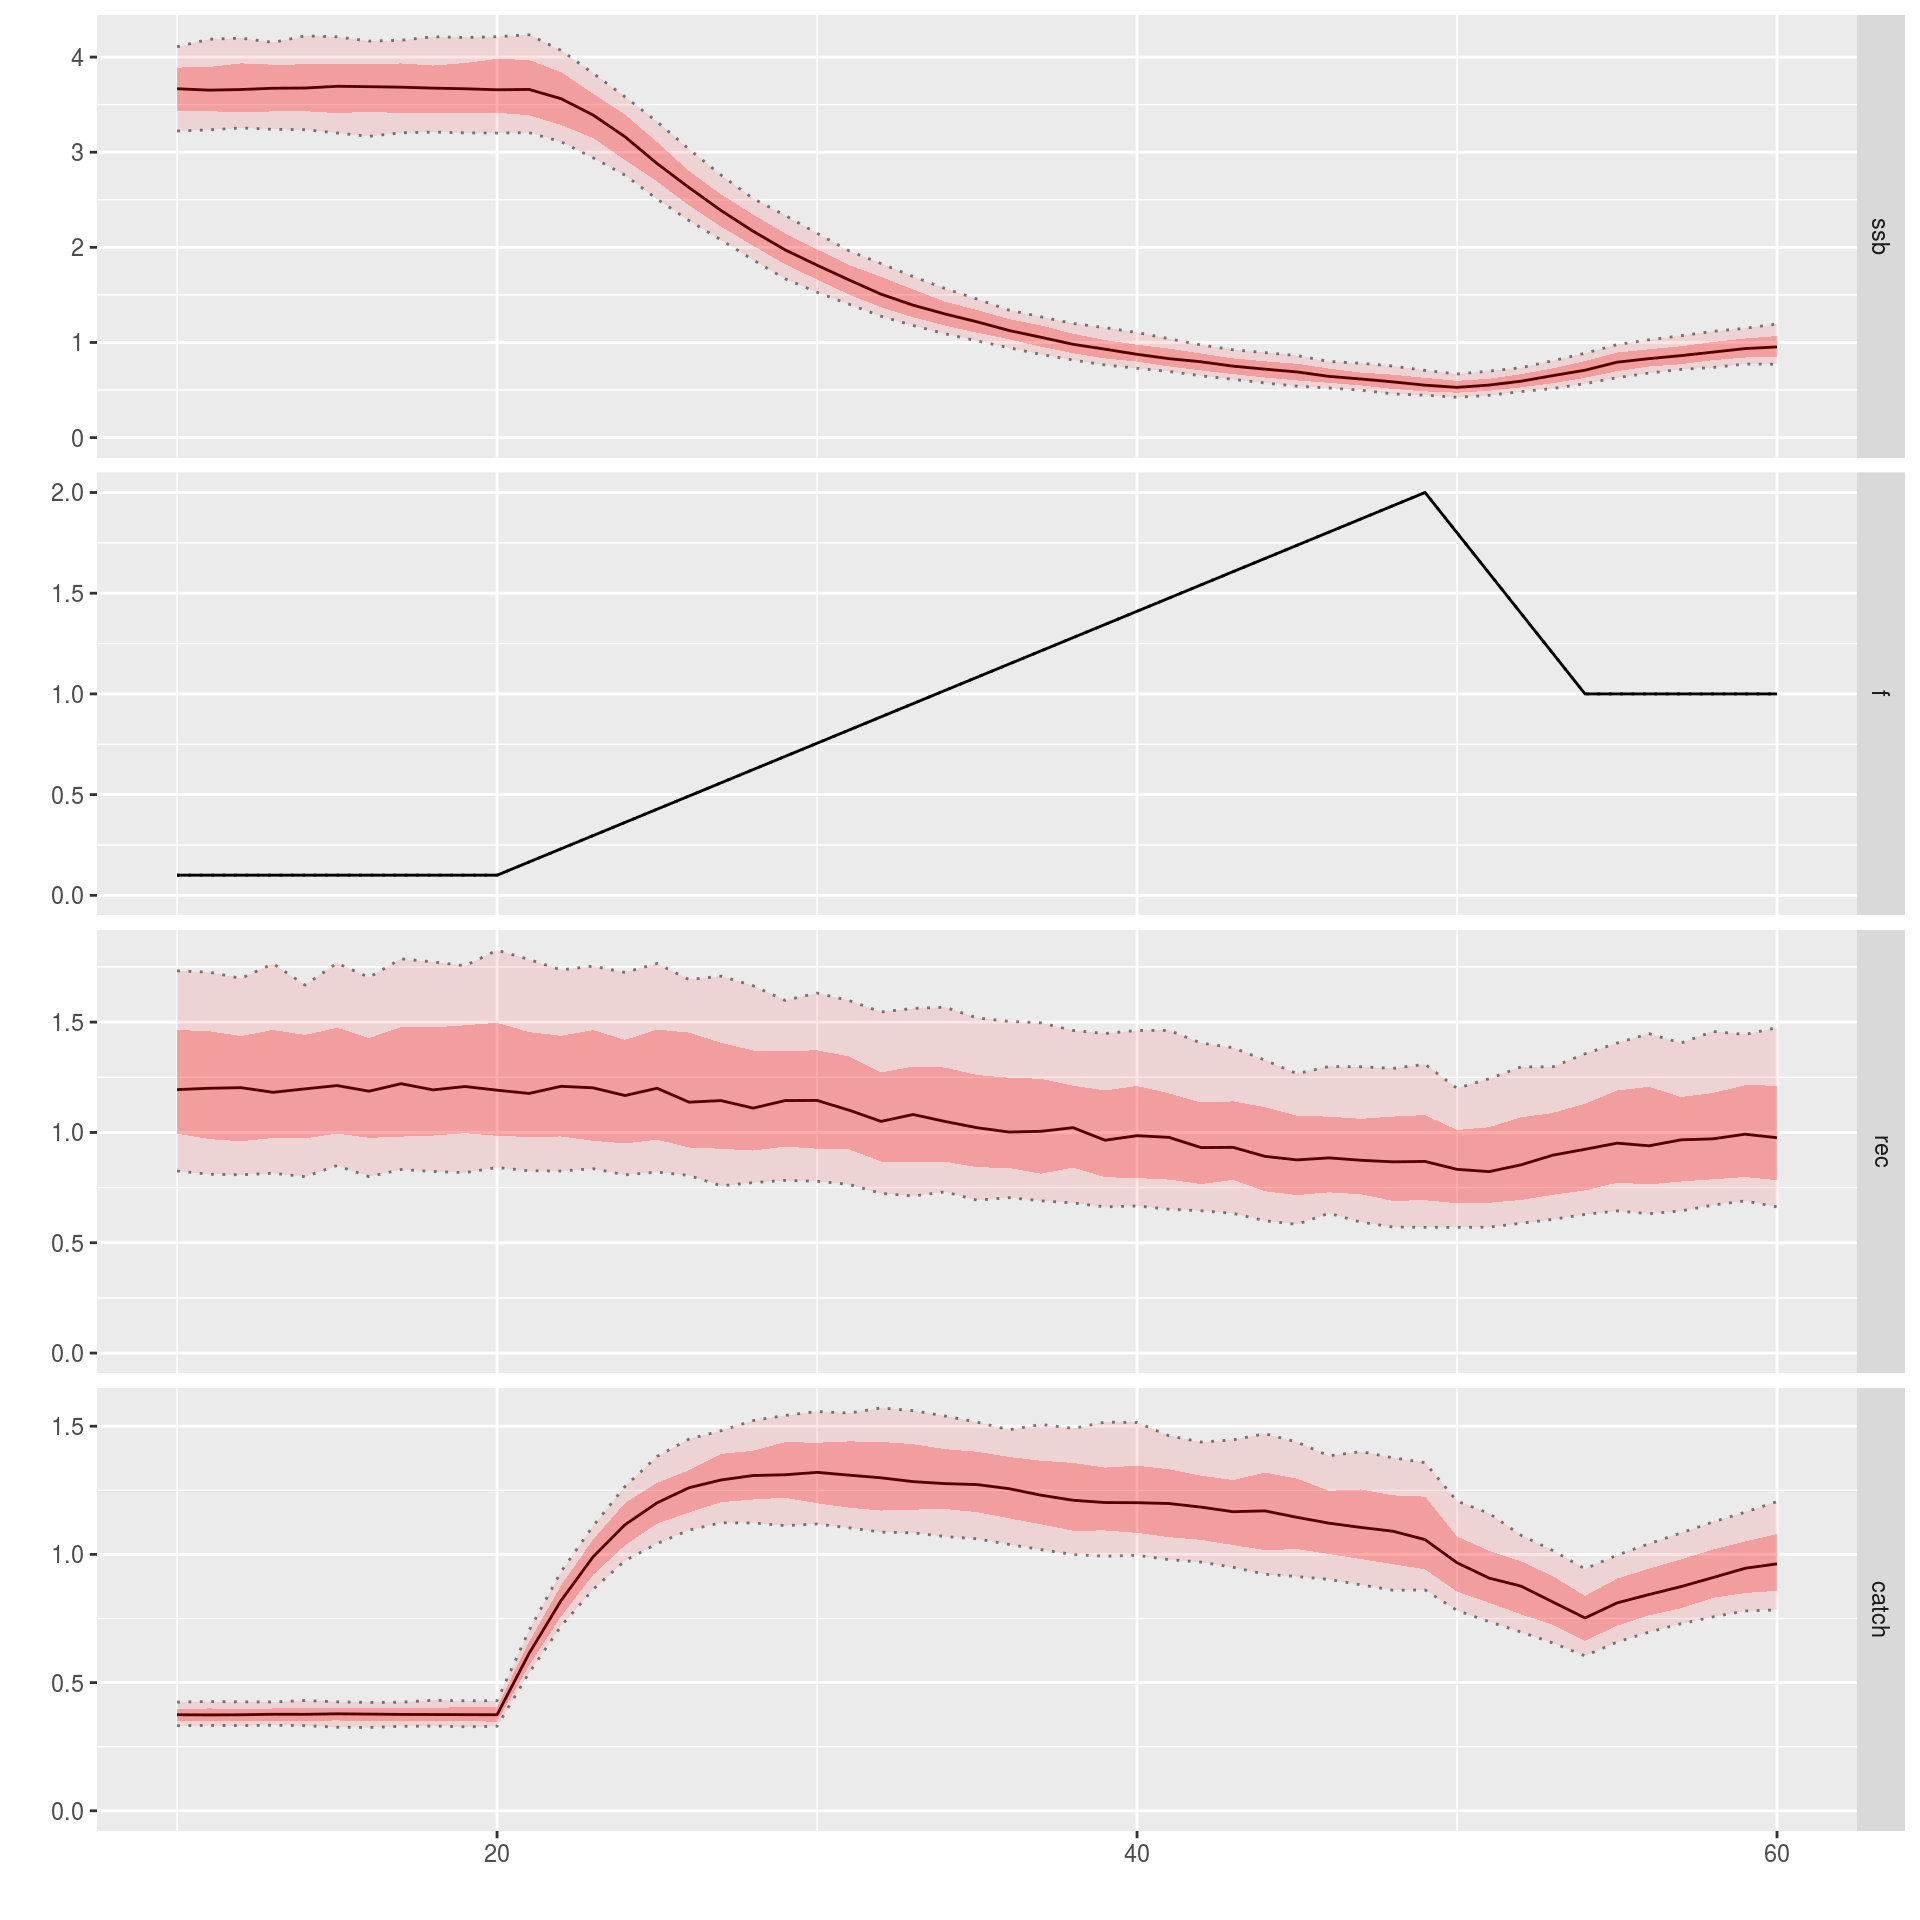
\includegraphics[width=5in]{rg-ts-1.png}\caption{}\label{fig:ts}\end{figure}
\begin{figure}[]\centering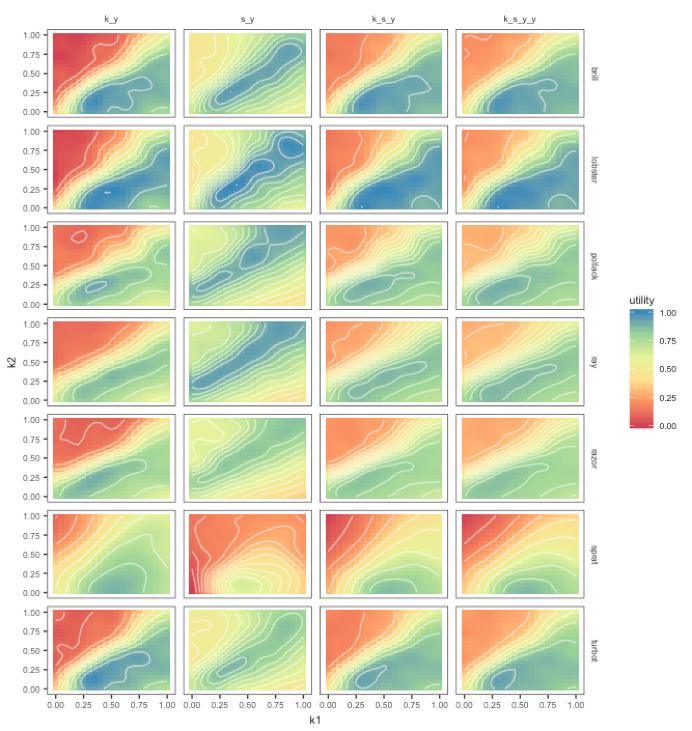
\includegraphics[width=5in]{util.png}\caption{}\label{fig:util}\end{figure}


%% Authors are advised to submit their bibtex database files. They are
%% requested to list a bibtex style file in the manuscript if they do
%% not want to use model1-num-names.bst.

%% References without bibTeX database:

% \begin{thebibliography}{00}

%% \bibitem must have the following form:
%%   \bibitem{key}...
%%

% \bibitem{}

% \end{thebibliography}


\end{document}

%%
%% End of file `elsarticle-template-1-num.tex'.